\section{Introduction}

Learning compact dynamical models is central to scientific machine learning when
high-fidelity simulation is too expensive for repeated evaluation. The problem is
especially difficult when a physical parameter changes the qualitative dynamics, not
only the response magnitude. Parameterized incompressible flows are representative:
different parts of the parameter domain may relax to a steady state, exhibit weak
oscillatory growth near instability onset, or sustain nonlinear periodic motion. A
many-query reduced model must remain accurate under autonomous rollout across all of
these regimes. Unlike a snapshot interpolant, it must continue evolving after the short
initial history is exhausted, without injecting reference states into the prediction
window.

Broad parameter ranges create two coupled difficulties. First, the state representation
is regime dependent: a basis that efficiently describes nearly steady states need not
compactly represent developed periodic dynamics. Second, the reduced evolution law must
reproduce distinct mechanisms such as decay, growth, phase evolution, and saturation.
A global model must solve both problems simultaneously, while recursive prediction
continually feeds its own errors back into the dynamics. The difficulty is therefore not
only model capacity: global coordinates can spend dimensions reconciling distinct state
geometries, and one global evolution law can average mechanisms that should remain
regime specific.

Projection-based reduced-order models provide explicit low-dimensional structure through
POD and Galerkin projection \citep{sirovich1987,berkooz1993,benner2015}, but truncated
interactions can degrade closure and long-horizon behavior \citep{amsallem2012}.
Learned dynamics offer richer nonlinear maps, yet one-step accuracy need not survive
recursive use \citep{pathak2018,vlachas2018,duraisamy2019,brunton2020}. Hybrid methods
therefore combine a projected backbone with learned unresolved terms
\citep{dar2023,lee2020,fresca2022,geelen2023}. A complementary approach replaces one
global representation with local subspaces, clusters, or manifolds
\citep{kaiser2014,li2021cluster,diaz2024}. These two remedies address complementary
parts of the problem---the first improves the dynamical inductive bias, while the second
reduces representation mismatch.

Localization, however, creates an assembly problem. Independently constructed charts
have different affine means, bases, scalings, and reduced operators, so their coefficient
vectors have no canonical componentwise correspondence. Switching or averaging those
vectors can therefore mix incompatible representations. Mixture-of-experts (MoE) models
provide a natural language for conditional computation
\citep{jacobs1991,jordan1994,shazeer2017,fedus2022}, but conventional MoE layers typically
route predictors acting in a shared feature space. Regime-dependent reduced dynamics
instead require both conditional closure within a chart and selection or combination of
complete autonomous models across noncommensurate charts. The outer decision must also
respect which local models are supported near a regime boundary; router confidence alone
does not make a cross-chart combination dynamically meaningful.

We introduce the \emph{Regime-Adaptive Localized Mixture-of-Experts Reduced-Order Model}
(RAL-MoE-ROM), a two-level hierarchy for this setting. Overlapping regime-local charts
each support an autonomous physics--data specialist. Within a specialist, hierarchical
sparse routing selects structured correction experts with nonlinear, affine, and
low-rank bilinear branches while retaining the projected dynamics as an explicit
inductive bias. Group Top-1 and channel Top-2 decisions activate a shared expert and a
small routed subset for the velocity and pressure channels. Specialists are trained with
closed-loop multi-step objectives so that the learned correction is exposed to its own
recursive inputs. Across specialists, a parameter-only E2 router produces one
trajectory-level regime preference. Physical-history descriptors are used only by the
Top-2 convex correction (T2-C) in an admissible overlap. The two selected specialists
encode the same physical history in their native charts, evolve independently, and are
combined only after reconstruction on the common physical mesh. The fused field is an
output and is never fed back into either local rollout.

Our contributions are threefold:
\begin{itemize}
    \item \textbf{Two-level hierarchical routing.} Sparse expert routing models
    unresolved dynamics inside each local specialist, while a second level selects or
    combines complete specialists across regimes. This distinguishes conditional closure
    from conditional selection of an entire dynamical system.

    \item \textbf{Structured closures for autonomous reduced dynamics.} Nonlinear,
    affine, and low-rank bilinear expert branches augment an explicit projected backbone
    and are trained under closed-loop rollout. Separate velocity and pressure routing
    allows the two algebraically different correction channels to adapt independently.

    \item \textbf{Physical-space assembly of noncommensurate local models.} Adjacent
    specialists retain independent coordinates and rollouts; T2-C couples only their
    reconstructed fields, avoiding coefficient or operator interpolation. A learned
    history-conditioned correction refines the parameter-only routing preference while
    preserving a convex output.
\end{itemize}

\begin{figure}[t]
    \centering
    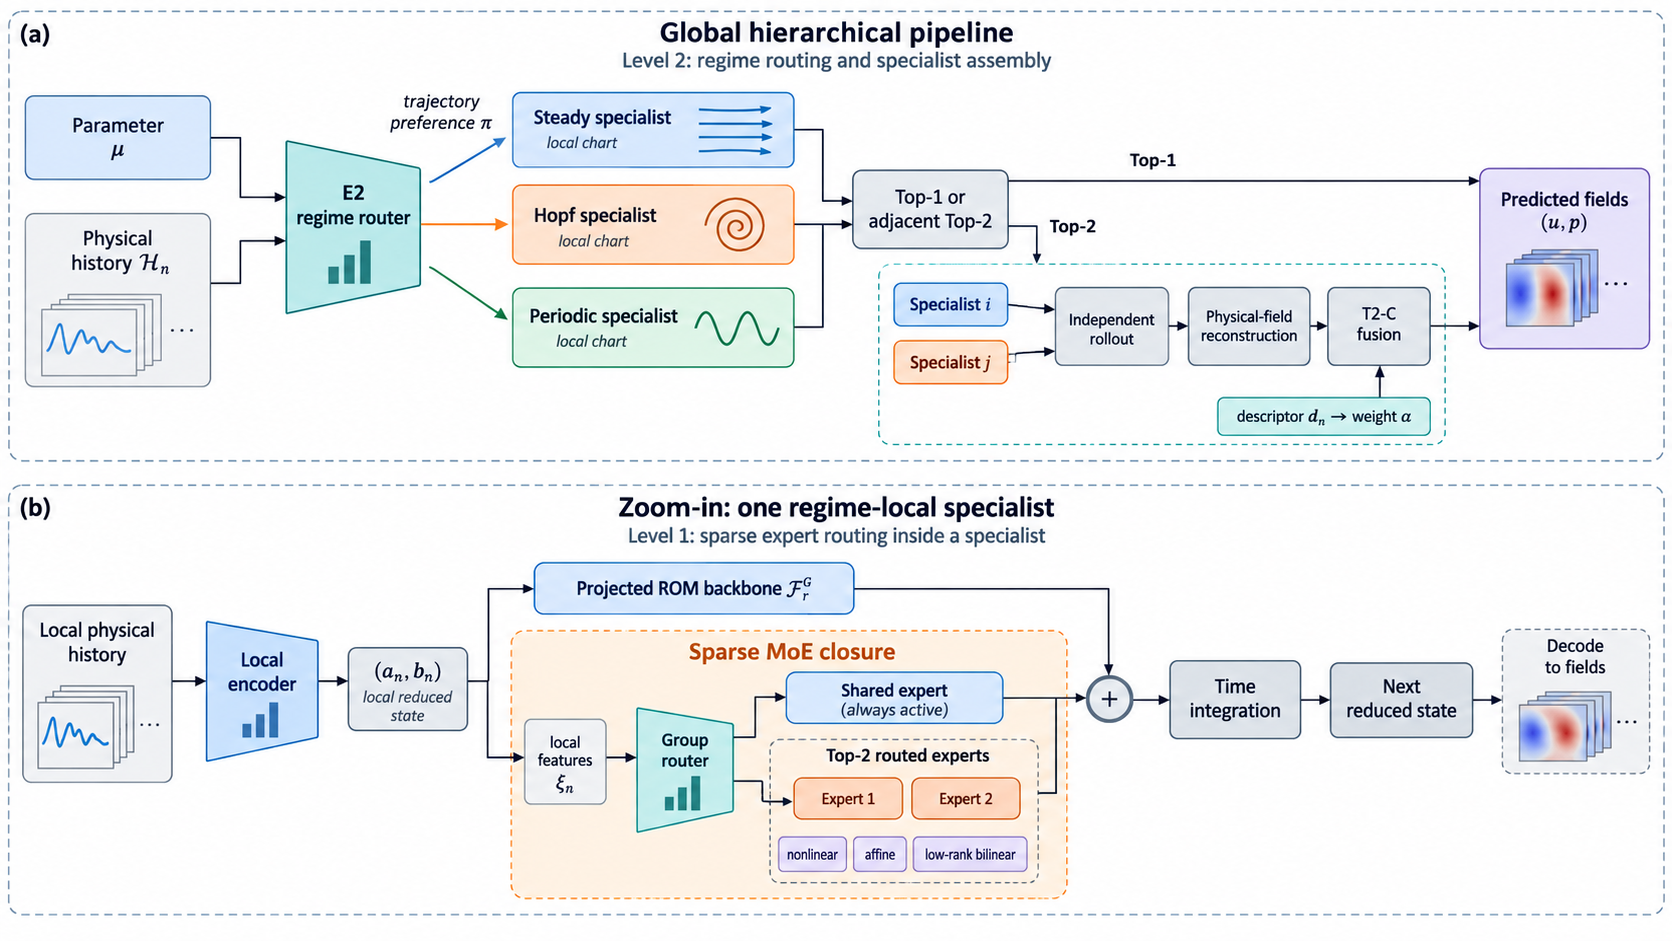
\includegraphics[width=\linewidth]{figures/ral_moe_rom_framework_user.png}
    \caption{Two-level RAL-MoE-ROM overview. (a) Regime-local specialists evolve
    independently and are combined after physical-field reconstruction.
    The history connection denotes access by the overall assembly: history
    initializes specialists and conditions T2-C, whereas E2 uses only $\mu$
    to produce the trajectory-level preference $\bm\pi$.
    (b) Sparse closure within a specialist, with a shared expert active in the
    selected group and channel-specific Top-2 routed experts. The update is
    schematic; pressure uses the algebraic map in Appendix~\ref{app:specialists}.}
    \label{fig:ral_overview}
\end{figure}

We evaluate RAL-MoE-ROM on three parameterized incompressible-flow systems spanning
steady, Hopf-onset, and periodic dynamics. The experiments separate the effects of the
structured expert map, projected backbone, localization, and cross-regime assembly. Over
the evaluated finite horizons, the local specialists remain accurate and finite, and
T2-C improves the corresponding hard or single-specialist prediction in the tested
overlaps. The comparisons include vanilla experts, data-only dynamics, a global chart,
POD--Galerkin, one-step POD--DeepONet, hard routing, and fixed or probability-based
blends. Localization is not uniformly superior to a global model at every parameter;
its value emerges from combining local coordinates, regime-specific dynamics, and
adaptive assembly.
